\documentclass[a4paper, 12pt]{article}
\usepackage[margin=1in]{geometry}
\usepackage{graphicx}
\usepackage{amsmath, amsthm, amssymb, amsfonts}
\usepackage{fancyhdr}
\usepackage{tikz}
\usepackage{parskip}
\usepackage{float}
\usepackage{enumitem}
\usepackage{array}

\usetikzlibrary{automata, positioning, arrows}

\setlength{\headheight}{14.49998pt}

\tikzset {
    ->,
    >=stealth',
    node distance=3cm,
    every state/.style={thick, fill=gray!10},
    initial text = $ $
}

\makeatletter
\renewenvironment{proof}[1][\proofname]{\par
%  \pushQED{\qed}% <--- remove the QED business
  \normalfont \topsep6\p@\@plus6\p@\relax
  \trivlist
  \item[\hskip\labelsep
        \itshape
    #1\@addpunct{.}]\ignorespaces
}{%
%  \popQED% <--- remove the QED business
  \endtrivlist\@endpefalse
}
\renewcommand\qedhere{} % to ensure code portability
\makeatother

\pagestyle{fancy}
\fancyhead[l]{SECJ3203}
\fancyhead[c]{Tutorial 7}
\fancyhead[r]{23 May 2025}

\title{Tutorial 7 & 8}
\date{}
\author{}

\renewcommand{\proofname}{Solution:}

\begin{document}
    \begin{enumerate}
        \item Let $M$ be the PDA as follows.
        
        \begin{center}
            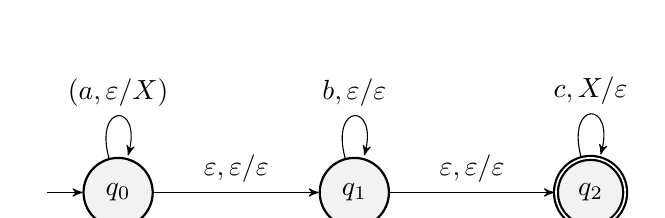
\begin{tikzpicture}
                \node[state, initial] (q0) {$q_0$};
                \node[state, right of=q0] (q1) {$q_1$};
                \node[state, accepting, right of=q1] (q2) {$q_2$};

                \draw 
                (q0) edge[loop above] node{$(a, \varepsilon/X)$} (q0)
                (q0) edge[above] node{$\varepsilon, \varepsilon/\varepsilon$} (q1)
                (q1) edge[loop above] node{$b, \varepsilon/\varepsilon$} (q1)
                (q1) edge[above] node{$\varepsilon, \varepsilon/\varepsilon$} (q2)
                (q2) edge[loop above] node{$c, X/\varepsilon$} (q2s);
            \end{tikzpicture}
        \begin{enumerate}
            \item Give the transition table of $M$.
                \begin{proof}
                    \leavevmode
                    \begin{center}
                        \begin{tabular}{|c|c|c|c|c|}
                            \hline
                            $\delta$ & $a$ & $b$ & $c$ & $\varepsilon$ \\
                            \hline
                            $q0$ & $q0, \varepsilon/X$ & - & - & $q1, \varepsilon/\varepsilon$ \\
                            \hline
                            $q1$ & - & $q1, \varepsilon/\varepsilon$ & - & $q2, \varepsilon/\varepsilon$ \\
                            \hline
                            $q2$ & - & - & $q2, X/\varepsilon$ & - \\
                            \hline
                        \end{tabular}
                    \end{center}
                \end{proof}
            \item Trace all computations of strings $ac, abbc, aabcc$ in $M$.
                \begin{proof}
                    \begin{align*}
                        (q_0, ac, \$) &\vdash (q_0, c, X\$) \\
                        &\vdash (q_1, c, X\$) \\
                        &\vdash (q_2, c, X\$) \\
                        &\vdash (q_2, \lambda, \$) 
                    \end{align*}
                    \begin{align*}
                        (q_0, abbc, \$) &\vdash (q_0, bbc, X\$) \\
                        &\vdash (q_1, bbc, X\$) \\
                        &\vdash (q_1, bc, X\$) \\
                        &\vdash (q_1, c, X\$) \\
                        &\vdash (q_2, c, X\$) \\
                        &\vdash (q_2, \lambda, \$)
                    \end{align*}
                    \begin{align*}
                        (q_0, aabcc, \$) &\vdash (q_0, abcc, X\$) \\
                        &\vdash (q_0, bcc, XX\$) \\
                        &\vdash (q_1, bcc, XX\$) \\
                        &\vdash (q_1, cc, XX\$) \\
                        &\vdash (q_2, cc, XX\$) \\
                        &\vdash (q_2, c, X\$) \\
                        &\vdash (q_2, \lambda, \$)
                    \end{align*}
                \end{proof}
            \item Give a set-theoretic definition of the language accepted by $M$.
                \begin{proof}
                    \(M = \{a^mb^nc^m \mid m, n \geq 0\}\)
                \end{proof}
            \item Write a grammar for the corresponding PDA.
                \begin{proof}
                    \begin{align*}
                        S &\to aSc \mid B \mid \lambda \\
                        B &\to bB \mid \lambda
                    \end{align*}
                \end{proof}
            \item Write the shortest string that is IN and NOT IN the language $L(M)$.
                \begin{proof}
                    \leavevmode \\
                    Shortest string IN $L(M)$: $\lambda$

                    Shortest string NOT IN $L(M)$: $a$
                \end{proof}
        \end{enumerate}
        \end{center}

        \item Given the language \(L(M) = \{a^mb^{2n}c^m \mid m, n \geq 0\}\)
        \begin{enumerate}
            \item Design a pushdown automata (PDA) that accept the language $L(M)$.
                \begin{proof}
                    \leavevmode

                    \begin{center}
                        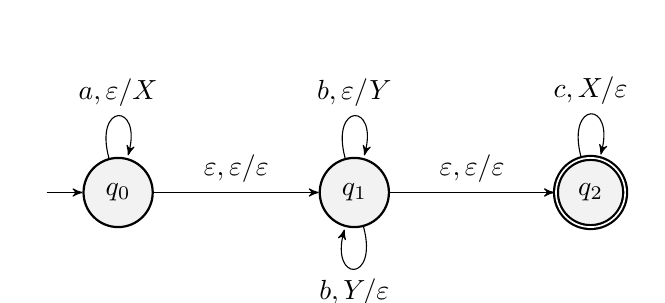
\begin{tikzpicture}
                            \node[state, initial] (q0) {$q_0$};
                            \node[state, right of=q0] (q1) {$q_1$};
                            \node[state, accepting, right of=q1] (q2) {$q_2$};

                            \draw
                            (q0) edge[loop above] node{$a, \varepsilon/X$} (q0)
                            (q0) edge[above] node{$\varepsilon, \varepsilon/\varepsilon$} (q1)
                            (q1) edge[loop above] node{$b, \varepsilon/Y$} (q1)
                            (q1) edge[loop below] node{$b, Y/\varepsilon$} (q1)
                            (q1) edge[above] node{$\varepsilon, \varepsilon/\varepsilon$} (q2)
                            (q2) edge[loop above] node{$c, X/\varepsilon$} (q2);
                        \end{tikzpicture}
                    \end{center}
                \end{proof}
            \item Trace the computation of the PDA that process the string $abbc$ and $abc$.
                \begin{proof}
                    \begin{align*}
                        (q0, abbc, \$) &\vdash (q0, bbc, X\$) \\
                        &\vdash (q1, bbc, X\$) \\
                        &\vdash (q1, bc, YX\$) \\
                        &\vdash (q1, c, X\$) \\
                        &\vdash (q2, c, X\$) \\
                        &\vdash (q2, \lambda, \$)
                    \end{align*}

                \begin{align*}
                    (q0, abc, \$) &\vdash (q0, bc, X\$) \\
                    &\vdash (q1, bc, X\$) \\
                    &\vdash (q1, c, YX\$) \\
                    &\vdash (q2, c, YX\$) \\
                    &\textit{Machine hangs...}
                \end{align*}
                \end{proof}
            \item What is the shortest string in the language accepted by the PDA.
                \begin{proof}
                    $\lambda$
                \end{proof}
        \end{enumerate}
    \end{enumerate}

    \newpage
    \fancyhead[c]{Tutorial 8}

    \begin{enumerate}
        \item Design a PDA for the following languages
        \begin{enumerate}
            \item \(\{a^{m+n}b^nc^m \mid m > 0, n \geq 0\}\)
                \begin{proof}
                    \leavevmode

                    \begin{center}
                        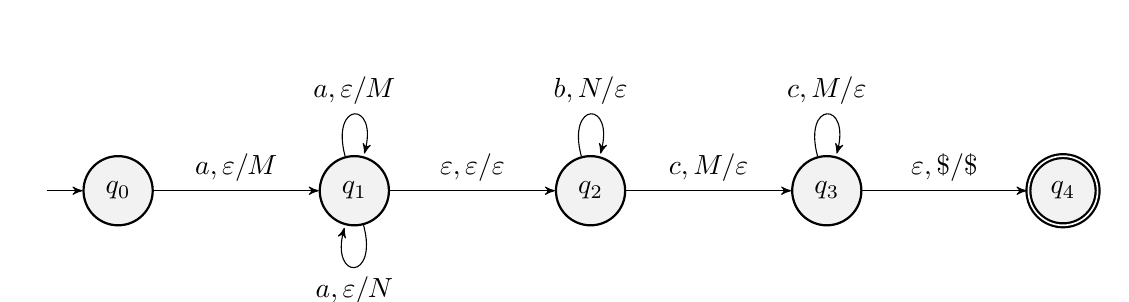
\begin{tikzpicture}
                            \node[state, initial] (q0) {$q_0$};
                            \node[state, right of=q0] (q1) {$q_1$};
                            \node[state, right of=q1] (q2) {$q_2$};
                            \node[state, right of=q2] (q3) {$q_3$};
                            \node[state, accepting, right of=q3] (q4) {$q_4$};

                            \draw
                            (q0) edge[above] node{$a, \varepsilon/M$} (q1)
                            (q1) edge[loop above] node{$a, \varepsilon/M$} (q1)
                            (q1) edge[loop below] node{$a, \varepsilon/N$} (q1)
                            (q1) edge[above] node{$\varepsilon, \varepsilon/\varepsilon$} (q2)
                            (q2) edge[loop above] node{$b, N/\varepsilon$} (q2)
                            (q2) edge[above] node{$c, M/\varepsilon$} (q3)
                            (q3) edge[loop above] node{$c, M/\varepsilon$} (q3)
                            (q3) edge[above] node{$\varepsilon, \$/\$$} (q4);
                        \end{tikzpicture}
                    \end{center}
                \end{proof}
            \item \(\{a^{m+n}b^nc^m \mid m \geq 0, n > 0\}\)
                \begin{proof}
                    \leavevmode

                    \begin{center}
                        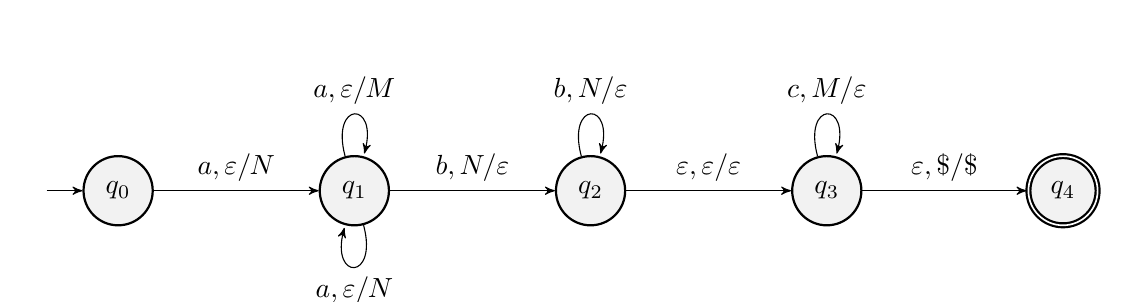
\begin{tikzpicture}
                            \node[state, initial] (q0) {$q_0$};
                            \node[state, right of=q0] (q1) {$q_1$};
                            \node[state, right of=q1] (q2) {$q_2$};
                            \node[state, right of=q2] (q3) {$q_3$};
                            \node[state, accepting, right of=q3] (q4) {$q_4$};

                            \draw
                            (q0) edge[above] node{$a, \varepsilon/N$} (q1)
                            (q1) edge[loop above] node{$a, \varepsilon/M$} (q1)
                            (q1) edge[loop below] node{$a, \varepsilon/N$} (q1)
                            (q1) edge[above] node{$b, N/\varepsilon$} (q2)
                            (q2) edge[loop above] node{$b, N/\varepsilon$} (q2)
                            (q2) edge[above] node{$\varepsilon, \varepsilon/\varepsilon$} (q3)
                            (q3) edge[loop above] node{$c, M/\varepsilon$} (q3)
                            (q3) edge[above] node{$\varepsilon, \$/\$$} (q4);
                        \end{tikzpicture}
                    \end{center}
                \end{proof}
            \item \(\{a^{m+n}b^nc^m \mid m, n \geq 0\}\)
                \begin{proof}
                    \leavevmode

                    \begin{center}
                        \begin{tikzpicture}
                            \node[state, initial] (q0) {$q_0$};
                            \node[state, right of=q1] (q1) {$q_1$};
                            \node[state, right of=q2] (q2) {$q_2$};
                            \node[state, accepting, right of=q2] (q3) {$q_3$};

                            \draw
                            (q0) edge[above] node{$\varepsilon, \varepsilon/\varepsilon$} (q1)
                            (q0) edge[loop above] node{$a, \varepsilon/M$} (q0)
                            (q0) edge[loop below] node{$a, \varepsilon/N$} (q0)
                            (q1) edge[above] node{$\varepsilon, \varepsilon/\varepsilon$} (q2)
                            (q1) edge[loop above] node{$b, N/\varepsilon$} (q1)
                            (q2) edge[above] node{$\varepsilon, \$/\$$} (q3)
                            (q2) edge[loop above] node{$c, M/\varepsilon$} (q2);
                        \end{tikzpicture}
                    \end{center}
                \end{proof}
            \item \(\{a^mb^nc^{m+n} \mid m, n > 0\}\)
                \begin{proof}
                    \leavevmode

                    \begin{center}
                        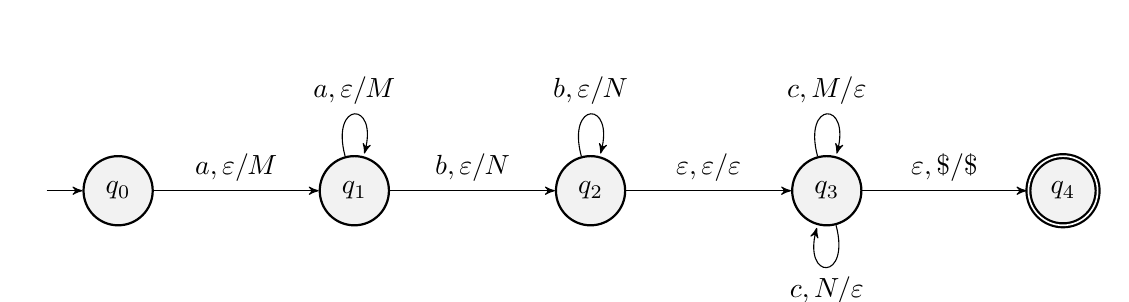
\begin{tikzpicture}
                            \node[state, initial] (q0) {$q_0$};
                            \node[state, right of=q0] (q1) {$q_1$};
                            \node[state, right of=q1] (q2) {$q_2$};
                            \node[state, right of=q2] (q3) {$q_3$};
                            \node[state, accepting, right of=q3] (q4) {$q_4$};

                            \draw
                            (q0) edge[above] node{$a, \varepsilon/M$} (q1)
                            (q1) edge[loop above] node{$a, \varepsilon/M$} (q1)
                            (q1) edge[above] node{$b, \varepsilon/N$} (q2)
                            (q2) edge[loop above] node{$b, \varepsilon/N$} (q2)
                            (q2) edge[above] node{$\varepsilon, \varepsilon/\varepsilon$} (q3)
                            (q3) edge[loop above] node{$c, M/\varepsilon$} (q3)
                            (q3) edge[loop below] node{$c, N/\varepsilon$} (q3)
                            (q3) edge[above] node{$\varepsilon, \$/\$$} (q4);
                        \end{tikzpicture}
                    \end{center}
                \end{proof}
            \item \(\{a^mb^nc^{m+n} \mid m, n \geq 0\}\)
                \begin{proof}
                    \leavevmode

                    \begin{center}
                        \begin{tikzpicture}
                            \node[state, initial] (q0) {$q_0$};
                            \node[state, right of=q1] (q1) {$q_1$};
                            \node[state, right of=q2] (q2) {$q_2$};
                            \node[state, accepting, right of=q2] (q3) {$q_3$};

                            \draw
                            (q0) edge[above] node{$\varepsilon, \varepsilon/\varepsilon$} (q1)
                            (q0) edge[loop above] node{$a, \varepsilon/M$} (q0)
                            (q1) edge[above] node{$\varepsilon, \varepsilon/\varepsilon$} (q2)
                            (q1) edge[loop above] node{$b, \varepsilon/N$} (q1)
                            (q2) edge[above] node{$\varepsilon, \$/\$$} (q3)
                            (q2) edge[loop above] node{$c, M/\varepsilon$} (q2)
                            (q2) edge[loop below] node{$c, N/\varepsilon$} (q2);
                           
                        \end{tikzpicture}
                    \end{center}
                \end{proof}
        \end{enumerate}
    \end{enumerate}
\end{document}